

%%-----------------------------------------------------
%%-----------------------------------------------------
\section{IFTTT - If This Then That}


%-----------------------    ---------------------------------

\begin{frame}
\frametitle{¿Qué es IFTTT?}

\begin{itemize}
   \item Servicio web que permite enlazar condiciones sencillas (recetas) y que realizan cambios en otros servicios web
   \item Ejemplos:
   \begin{enumerate}
     \item Cuando llegue a casa/trabajo, activa la wifi
     \item Baja el volumen del teléfono cuando esté en clase
     \item Cada vez que envíe un tweet, guárdamelo en Google Docs
     \item Si me etiquetan en Facebook, guarda una copia en Instagram
     \item Enciende las luces cuando entre por el garaje
   \end{enumerate}
\end{itemize}

\end{frame}


%-----------------------    ---------------------------------

\begin{frame}
\frametitle{IFTTT}

\begin{center}
  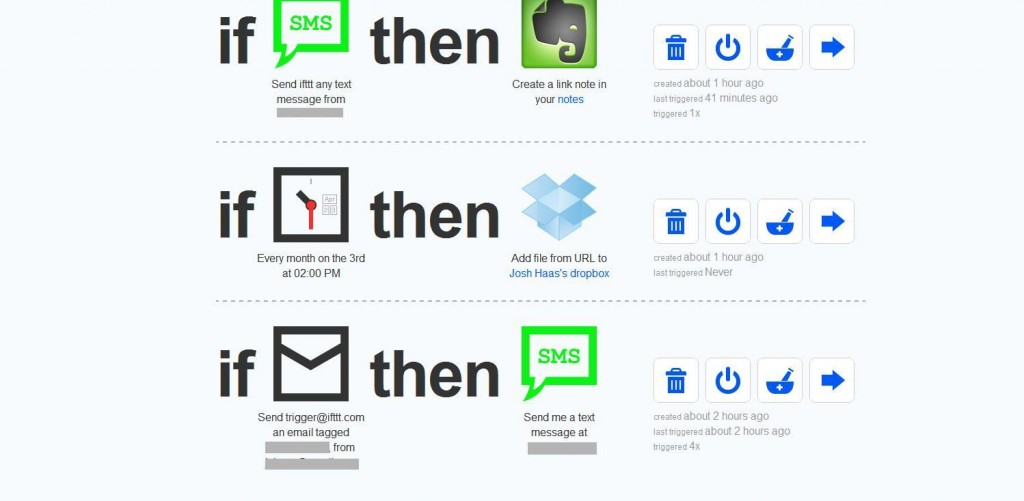
\includegraphics[width=13cm]{figs/if-recipes.jpg}
\end{center}


\begin{flushright}
{\tiny
Source: http://blog.joshhaas.com/2011/10/self-experimentation-using-ifttt-and-a-dash-of-python/
}
\end{flushright}

\end{frame}


%-----------------------    ---------------------------------

\begin{frame}
\frametitle{¿Por qué es interesante?}

\begin{itemize}
   \item La web no es sólo para humanos...
   \item Es un entorno distribuido multi-servicio
   \item Está adaptado al Internet de las cosas 
\end{itemize}

\end{frame}




